\documentclass[10pt,a4paper]{article}
\usepackage{caratula}
\usepackage{geometry}
\renewcommand\familydefault{\sfdefault} % Default family: serif 
\usepackage[usenames,dvipsnames]{xcolor}
\usepackage{tikz}
\usepackage{soul}
\usetikzlibrary{calc} 
\usetikzlibrary{arrows, decorations.markings,positioning,backgrounds,shapes}
\definecolor{EMP}{HTML}{77DD77} % Green1
\definecolor{NOR}{HTML}{06500C} % Green2
\usepackage{ulem}
\renewcommand{\ULdepth}{3pt}
\usepackage{tikz-dependency}
\usepackage{graphicx} 
\usepackage{indentfirst}
\setlength{\parindent}{12pt}
\usepackage{amsmath}


%\usetikzlibrary{positioning}




\titulo{TP1 }
\subtitulo{Relación PBI - Cantidad de sedes Argentinas en el exterior}

\fecha{\today}

\materia{Laboratorio de Datos}
\grupo{GRUPO 100}

\integrante{Chapana Puma, Joselin Miriam}{1197/21}{yoselin.chapana@gmail.com}
\integrante{Martinelli, Lorenzo}{364/23}{martinelli.lorenzo12@gmail.com}
\integrante{Padilla, Ramiro Martin}{1636/21}{ramiromdq123@gmail.com}

\graphicspath{{../static/}}


\begin{document}
\newgeometry{margin=2cm}

\maketitle

\restoregeometry
%\newgeometry{top=3cm,bottom=3cm,right=3cm,left=3cm} para editar margenes menos del titulo 


\section{Resumen} \vspace{0.3cm}

Estuve pensando y aca podriamos contar que fuimos pensando a lo largo del trabajo, los problemas con los que nos encontramos y como fue la dinámica, mas que nada porque la explicacion de la metodologia a seguir está en la parte de introducción.

\section{Introducción} \vspace{0.1cm}

\subsection{Objetivo y Fuente} \vspace{0.3cm}

El objetivo principal de este trabajo es encontrar una relación entre la cantidad de sedes de Argentina en un país y su PBI, si este será mayor, menor o si influirá la cantidad de secciones que una sede posea.  Para esto, trabajaremos con los siguientes datos, 

\begin{itemize}
	\item PBI per cápita de los paises (1)
	\item Representaciones Argentinas en el exterior, donde tenemos, Datos básicos de las sedes, Datos completos de sedes y secciones (2)
\end{itemize}

\noindent (1) Extraido de la pagina del Banco Mundial, https://data.worldbank.org/indicator/NY.GDP.PCAP.CD \\

\noindent (2) Obtenidas del Ministerio de Relaciones Exteriores, Comercio Internacional y Culto, \\ https://datos.gob.ar/dataset/exterior-representaciones-argentinas \vspace{0.1cm}
 
\subsection{Procedimiento} \vspace{0.3cm}

\indent Este trabajo tendrá varias etapas, comenzando con el planteo de un Diagrama de Entidad Relacional (DER) adecuado al objetivo de nuestro trabajo, es decir, a partir de los datasets mencionados anteriormente, nos quedaremos solo con aquellos datos necesarios para resolver nuestro problema. Luego, pasaremos nuestro DER al modelo relacional, el cual se encontrará en tercera forma normal y especificará claves primarias (PK), claves candidatas (CK), claves foráneas (FK) y dependencias funcionales. \par
Una vez tengamos nuestro modelo planteado, pasaremos a Python donde realizaremos una limpieza de los datos tomando ciertas decisiones que estarán explicadas hacia el final de este informe. 
Finalmente, con los datos ya limpios, a traves de distintas librerias como Pandas, Matplotlib, Inlinesql, entre otras nos encargaremos de consultar, manipular y visualizar los datos necesarios para dar con nuestro objetivo.


\newpage

\section{Procesamiento de Datos} \vspace{0.2cm}

Antes de comenzar con el procesamiento de datos, nos encontramos con las fuentes de datos originales en distintas formas normales. Comenzando con \textbf{lista-sedes-datos} y \textbf{lista-secciones}, tenemos que ninguna de ambas se encuentra en primera forma normal puesto que el atributo \textit{redes-sociales} de la primera y, el atributo \textit{telefonos\_principales} de la segunda tienen valores no atómicos. Al no estar en 1FN, tampoco se encontraran en 2FN. \par
Por otro lado, la tabla que contiene el pbi de los paises, está en primera y segunda forma normal, sin embargo no se encuentra en tercera forma normal puesto que tiene dependencias transitivas, en particular, la DF \{Country Code $\rightarrow$ Indicator Name\} es transitiva mediante el atributo \textit{Indicator Code}, el cual no es clave candidata pero forma parte de la DF \{Indicator Code $\rightarrow$ Indicator Name\}, ademas tomamos \textit{Country Code} como unica clave.  \par
Y, por último, la tabla \textbf{lista-sedes} está en segunda forma normal, pero no está en tercera forma normal puesto que tiene dependencias transitivas como por ejemplo, la DF \{sede\_id $\rightarrow$ pais\_iso\_2\} es transitiva mediante el atributo \textit{pais\_iso\_3}. Esto es asi por que consideramos \textit{sede\_id} como clave primaria

\subsection{Limpieza de Datos}

Buscando mejorar la calidad de datos, encontramos problemas de instancia, por ejemplo, datos inconsistentes, problemas de 
proceso, puesto que hay diferentes criterios en la carga de los datos. Ahora, veamos cada dataset en detalle,

\begin{enumerate}
	\item lista-sede-datos, en ella, encontramos un problema asociado a instancia en el atributo \textit{'redes\_sociales'} que influye en su consistencia puesto que no encontramos un criterio unificado a la hora de cargar distintas redes sociales. Por ejemplo, tenemos datos cargados en forma de URL donde es facil identificar a que red social pertenece, y por otro lado, tenemos datos que contienen, intuimos, nombres de usuarios, pero no podemos discernir su red social. Para tener una medida concreta acerca de la magnitud del problema utilizamos el método GQM de la siguiente manera:
\begin{itemize}
	\item Goal : Evitar que haya datos que no se puedan identificar con alguna red social.
	\item Question : ¿Cual es la cantidad de elementos en redes\_sociales que no podemos identificar?
	\item Metrica :  Proporción de registros sin campo redes\_sociales que son Urls o comienzan con @.
        
        \begin{center}          
        M1: $ \frac{\text{Cantidad de registros con datos en redes\_sociales que no son Urls o comienzan con @} }{\text{Cantidad de registros totales}} $
        \end{center}
    %(0.23)
    
\end{itemize}
Para corregir esta tabla, además, seleccionamos columnas que consideramos relevantes para la resolución de nuestro problema principal. Puesto que encontramos datos redundantes, como dos nomenclaturas de codigo (pais\_iso\_3 / pais\_iso\_2) para un mismo pais, o la traducción al inglés de los nombres de estos paises. También, consideramos mantener unicamente los datos de redes sociales que eran consistentes, es decir, que eran Urls o comenzaban con @.

Una vez hecha la limpieza de datos, procedemos a comparar las metricas antes y despues de dicha limpieza:
\begin{itemize}
    \item Antes: $M1 =  0.23$, es decir que un $\% 23$ de registros son no deseados
    \item Después: $M1 =  0$, es decir que un $\% 0$ de registros son no deseados
\end{itemize}

	\item En tabla correspondiente al PBI, API\_NY.GDP.PCAP.CD\_DS2\_en\_csv\_v2\_73.csv, tenemos también un problema de instancia, que afecta en particular, la completitud del atributo '2022'. Asi como también, otro problema de instancia es que encontramos muchos datos que no corresponden a paises. Estos fueron descartados antes de elaborar la siguiente métrica,
\begin{itemize}
	\item Goal : Tener el dato '2022' que refiere al Pbi de cada país completo.
	\item Question : ¿Es relevante la proporción de paises con el dato '2022' vacío?
	\item Metric: Proporción de paises con el campo '2022' vacío.
        \begin{center}
            M1: $\frac{\text{Cantidad de registros con dato vacio en el campo '2022'}}{\text{Cantidad de registros totales}}$
        \end{center}
  %(0.09)
\end{itemize}
Para corregir este dataset, en primeria instancia, descartamos todas las columnas que no aportaban a nuestro objetivo, como por ejemplo, 
todas aquellas correspondientes a años anteriores a 2022. En segunda instancia, eliminamos aquellos datos que no correspondian con paises, 
por ejemplo 'Africa'. 

Una vez hecha la limpieza de datos, procedemos a comparar las metricas antes y despues:

\begin{itemize}
    \item Antes: $M1 =  0.09$, es decir, un $\% 9$ de registros contienen NULL en el campo '2022'
    \item Después: $M1 =  0$, es decir, un $\% 0$ de registros son no deseados
\end{itemize}

En último lugar, consideramos que al ser tan baja la proporcion de nulls, era conveniente descartarlos. 

	\item Por último, en lista-secciones, nos quedamos unicamente con las dos primeras columnas, sede\_id y descripción, en las cuales no encontramos ningun problema de calidad.
\end{enumerate}

\newpage
\subsection{Diagrama de Entidad Relacional} \vspace{0.2cm}

Una vez planteado nuestro objetivo, nos encargamos de ver que datos necesitabamos para alcanzarlo, y como estarian representados. Para esto, elaboramos el siguien diagrama de entidad
relacional.  \vspace{0.2cm}

\begin{figure}[ht]
	\centering
	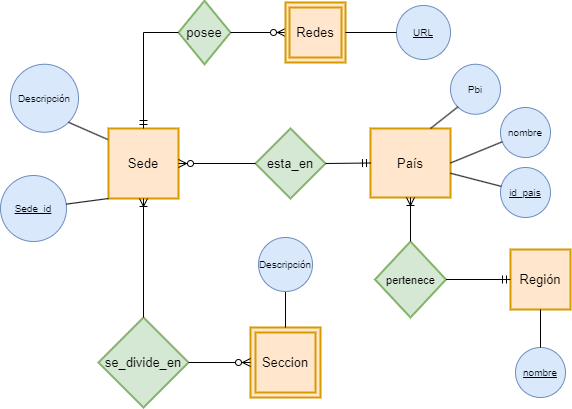
\includegraphics[width=1\textwidth]{DerFinal.png}
	\caption{Diagrama de Entidad Relacional}
	\label{fig:ejemplo}
\end{figure} \vspace{0.1cm}

Como se puede ver en la imagen anterior, consideramos que,

\begin{itemize}
	\item Una sede esta en un país y solo en uno.
	\item Un País puede tener muchas o ninguna sede.
	\item Las secciones existen pues existen las sedes, entonces, lo consideramos una entidad debil.
	\item Una sección puede estar en una o muchas Sedes, por ejemplo, la Embajada en Brasil y en Chile tiene su sección Administración.
	\item Una sede tiene al menos una sección.
	\item Cuando hablamos de Redes, hablamos mas de un perfil en una red social, por lo tanto, una red puede pertenecer a una y solo una sede.
\end{itemize}


\subsection{Modelo Relacional} \vspace{0.2cm}

Una vez que tenemos nuestro esquema gráfico, pasamos al planteo del modelo relacional. Notar que, las flechas representan las Foreign Keys y aquellos atributos 
subrayados representan las Primary Keys. En todas las relaciones, exceptuando a País, las Claves coinciden con las claves candidatas, esto se debe a que en País consideramos también a 
nombrePais como una posible clave.  \vspace{0.4cm}

\newbox\ubox

\begin{tikzpicture}[
    EMP/.style={% Style for empatized boxes
        rectangle, line width =1pt,
        anchor=west,
        underline, % new property
        align=center,
        text=Black,
        minimum height=.8cm,
        text height=1.7ex,
            text depth=.25ex,
        fill=EMP,
        draw=black,
        },
    NOR/.style={% Style for normal boxes.
        rectangle, 
        line width =1pt,
        anchor=west,
        align=left,
        minimum height=.6cm,
        text height=1.5ex,
            text depth=.25ex,
            text=white,
        fill=NOR,
        draw=black,
        inner ysep=5pt
        },
    underline/.append style={% define new style property
        execute at begin node={%
            \setbox\ubox=\hbox\bgroup
            },
            execute at end node={%
                \egroup\uline{\box\ubox}%
                }
             },
    ] % Uff that is all the configuration for tickzpicture xD

% Define an brute force objet "Frame"
% Variables 1:Position, 2: Identifier, 3: Title of frame 4: Subframe/Boxtype
 \def\Frame(#1)#2[#3]#4{%
  \begin{scope}[shift={(#1)}] 
      \node[font=\bf, anchor=west] (Title) at (-0.2,0.7) {#3}; 
       \edef\k{0}% Variable for box positión
       \edef\x{0}% Variable for named coordinate centering - below box
       \foreach \id/\style in {#4} {%enter sub frame data Name/Boxtype ,Name2/Boxtype | An space before Boxtype is needed 
            \node[\style] (h) at (\k pt,0) {\id}; %  % Draw a node depending on the variables.
            \pgfmathparse{\k+0.5*width{"\id"}+3.4pt} % Uses the textwidth to calculate named coordinate  
            \xdef\x{\pgfmathresult} % The resul is saved in the variable \x
            \draw (\x pt,-0.4) coordinate (\id#2); %Create a named coordinate concatenated: "sub frame data Name"+"identifier"
            \pgfmathparse{\k+width{"\id"}+6.8pt}% Calculate positión for each subframe box.       
        \xdef\k{\pgfmathresult}% Save the value to be added to the next iteration value.
       }    
  \end{scope}
}% disadvantages: Is not posible to use Frame data Name like: Name_another_desc instead I use Name-another-desc

% Start drawing
% \node[EMP node] (dm) at (0,0) {{Sometext/EMP,another/EMP}};
  \Frame(0,0){3}[PAIS]{
    IdPais/EMP,
    NombrePais/NOR,
    Pbi/NOR};

 \Frame(0,-2.5){1}[SEDE]{%first frame identified as 1 named EMPLOYEE
    IdSede/EMP,% see that it is necessary to add a space
    IdPais/NOR,
    Descripción/NOR}; 

 \Frame(0,-5){2}[REDES]{
    IdSede/EMP,
    Urls/EMP};  

 \Frame(0,-7.5){4}[REGION]{
    IdPais/EMP,
    Region/NOR};

  \Frame(0,-10){5}[SECCIONES]{
    IdSede/EMP,
    SeccionDescripcion/EMP};     

% Start drawing arrows:
% In this part I use the named coordinates to draw the arrows.
    \draw[thick,<-,thick,>=latex] % From Essn6 to Ssn1  
        (IdSede1)++(0.1,0) -- ++(0,-.55) -- ++(4.5,0) coordinate (inter) %inter is the name of coordinate register
        -- (IdSede2 -| inter) -- ++(0,-0.4) coordinate (inter)  % to calculate intersections.
        -- (IdSede2 |- inter) --++(0,0.4); %
        
    \draw[thick,<-,thick,>=latex]
        (IdPais3) -- ++(0,-.675) -- ++(5.2,0) coordinate (inter) 
        -- (IdPais4 -| inter) -- ++(0,-0.2) coordinate (inter) 
        -- (IdPais4 |- inter) --++(0,0.2); %

     \draw[thick,<-,thick,>=latex]
        (IdSede1)++(-0.3,0) -- ++(0,-.85) -- ++(4.3,0) coordinate (inter) 
        -- (IdSede5 -| inter) -- ++(0,-0.2) coordinate (inter) 
        -- (IdSede5|- inter) --++(0,0.2); %.
        
     \draw[thick,<-,thick,>=latex]
        (IdSede1)++(-0.3,0) -- ++(0,-.85) -- ++(4.3,0) coordinate (inter) 
        -- (IdSede5 -| inter) -- ++(0,-0.2) coordinate (inter) 
        -- (IdSede5|- inter) --++(0,0.2); %.

    \draw[thick,<-,thick,>=latex] % From Essn6 to Ssn1  
        (IdPais3)++(0.2,0) -- ++(0,-.5) -- ++(5.2,0) coordinate (inter) %inter is the name of coordinate register
        -- (IdPais1 -| inter) -- ++(0,-0.4) coordinate (inter)  % to calculate intersections.
        -- (IdPais1 |- inter) --++(0,0.45); %

 
\end{tikzpicture} \vspace{0.4cm}

Ahora, solo resta mostrar las dependencias funcionales de este modelo relacional para dejar en claro que se encuentra en la forma normal deseada (3FN) y, también tener completo nuestro esquema para asi comenzar a manipular los datos.

\newpage

\subsection{Dependencias Funcionales} \vspace{0.1cm}

A continuación, mostramos las dependencias funcionales de las relaciones de nuestro modelo relacional. En esta, se puede apreciar que 
todas se encuentran en segunda y tercera formal. Luego, con la limpieza de datos, garantizaremos que todos sus atributos sean atómicos
y por ende se encuentre también en primera forma normal.  \vspace{0.3cm}

\depstyle{lvl}{%
    edge height=2.5ex,
    % edge unit distance=#1*2.5ex, % Another way of controlling the appearance of the edges.
    edge below,
    edge horizontal padding=0,
    edge vertical padding=(#1-1)*3ex,
    text only label, % No need for label for functional dependencies.
    edge slant=0, % Right angles
    rounded corners=0,
    edge style={>=triangle 60} % Change the style of the arrowheads.
}
\tikzset{
    matrix/.append style={column sep=0.4cm} % Adding some distance between the attributes.
}
\tikzstyle{TxtBook}=[% Style to mimic the textbook Fundamentals of Database Systems.
    column sep=0cm, % No distance between two attributes.
    nodes={%
        fill=gray!20,
        draw=black,
        thick,
        inner xsep=3ex,
        inner ysep=1ex
    }
]
\tikzstyle{TxtBookChico}=[% Style to mimic the textbook Fundamentals of Database Systems.
    column sep=0cm, % No distance between two attributes.
    nodes={%
        fill=gray!20,
        draw=black,
        thick,
        inner xsep=1.2ex,
        inner ysep=1ex
    }
]


\textbf{Sede} \vspace{0.1cm}

\begin{dependency}
    \raggedright
    \begin{deptext}[TxtBookChico] % Applying the TxtBook style.
        \textbf{\underline{idSede}}  \& idPaís \& Descripción\\
    \end{deptext}
    \depedge[lvl=1]{1}{2}{}
    \depedge[lvl=1]{1}{3}{}
\end{dependency} \vspace{0.3cm}
 \vspace{0.3cm}

\textbf{País} 
\vspace{0.1cm}

\begin{dependency}
    \raggedright
    \begin{deptext}[TxtBook] % Applying the TxtBook style.
        \textbf{\underline{idPaís}}  \& NombrePaís \&Pbi \\
    \end{deptext}
    \depedge[lvl=1]{1}{2}{}
    \depedge[lvl=1]{1}{3}{}
    \depedge[lvl=2]{2}{1}{}
    \depedge[lvl=2]{2}{3}{}
\end{dependency} \vspace{0.3cm}

\textbf{Región} 
\vspace{0.1cm}

\begin{dependency}
    \raggedright
    \begin{deptext}[TxtBook] % Applying the TxtBook style.
        \textbf{\underline{idPaís}} \& Región  \\
    \end{deptext}
    \depedge[lvl=1]{1}{2}{}
\end{dependency} 

\vspace{3mm}
\textbf{Sección} 

\begin{dependency}
    \raggedright
    \begin{deptext}[TxtBook] % Applying the TxtBook style.
        \textbf{\underline{IdSede}}  \& \textbf{\underline{Sección}}  \\
    \end{deptext}
    \depedge[lvl=1]{1}{2}{}
    \depedge[lvl=1]{2}{1}{}
\end{dependency} \vspace{0.1cm}

Observación: la única DF es $\{$IdSede, Sección$\} \rightarrow \{$IdSede, Sección$\}$

\vspace{3mm}
\textbf{Redes} 

\begin{dependency}
    \raggedright
    \begin{deptext}[TxtBook] % Applying the TxtBook style.
        \textbf{\underline{IdSede}}  \& \textbf{\underline{redURL}}  \\
    \end{deptext}
	\depedge[lvl=1]{2}{1}{}
\end{dependency} \vspace{0.3cm}

\subsection{Importación de Datos} \vspace{0.3cm}

Una vez ya limpios los datos, creamos con pandas un archivo csv para cada relación de nuestro modelo. Luego, los importamos 
a los dataframe vacíos creados anteriormente.

\section{Decisiones tomadas}

En los distintos procedimientos que llevamos acabo explicados en la sección anterior, encontramos necesario realizar tomas de decisiones para mejorar, mantener la calidad de datos y cumplir la normalización pedida en el informe. Esto debido a que encontramos atributos irrelevantes, que presentaban información confusa o datos ya presentados en otros atributos. Estas decisiones fueron las siguientes:
\begin{itemize}
    \item En la lista-sede-datos encontramos muchos registros con datos correspondientes al atributo "redes\_sociales" que no contaban con una forma consistente a la hora de cargarse. Por lo que, como fue explicado en la sección \textbf{3.1 Limpieza de datos}, mantuvimos los datos que efectivamente se podian deducir que eran URLs y aquellos que contenian "@" al principio. Esto último debido a que es la manera más frecuente de referirse a usuarios de una Red Social. En este caso especifico, tomamos la decisión de que estos casos sean adjudicados a la red social "Instagram". Consdieramos que, si los eliminamos, perdemos una cantidad importante de información.
    \item En el momento de crear el Diagrama de Entidad Relacioal y su correspondiente Esquema Relacional, tomamos la decisión de establecer como clave primaria aquellos atributos que son códigos. Por esto mismo, le dimos importancia a los id de las sedes en lugar de a su nombre. Asi también tomamos como clave el id de cada pais obtenida de la tabla que contenia los PBI de cada país, además porque en lista-sede-datos contamos con un atributo idéntico (pais\_iso\_3) que nos iba a permitir establecer una conexión entre tablas.
    \item Como en lista-sedes-datos encontramos la misma cantidad de registros y la misma información que en lista-sedes, tomamos la decisión de utilizar la primera tabla ya que contiene más atributos, y por ende, más información necesaria para analizar.
% tambien pense en agrergar pq eliminamos nulls de pbi, pero ya lo dijimos antes, no sé
\end{itemize}

\newpage

\section{Análisis de datos}

\subsection{Consultas SQL}

Para el analisis de datos, se elaboraron una serie de tablas mediante consultas SQL.

En primer lugar, se consideraron la cantidad de sedes, el número promedio de secciones por sede y el PBI per cápita correspondiente al año 2022 de cada país.
De acuerdo con los resultados obtenidos en la tabla "pais\_seccciones.csv" (consulte el Anexo para visualizarla), se destaca que Brasil y Estados Unidos son los países con mayor número de sedes, con PBIs de 8918 y 76330, respectivamente. Además, se observa que Mónaco, con un PBI de 240862, y Burundi, con un PBI de 259, son los países con el mayor y el menor PBI, respectivamente, a pesar de no tener sedes. Esto nos hace dudar, en que infulirá la cantidad de sedes argentinas.

\vspace{0.1cm}

En una segundo lugar, se analizó la tabla "region\_pais\_pbi", que incluye información sobre la cantidad de paises con alguna sede en distintas regiones geográficas y el promedio de su Pbi. Se destaca que Oceanía es la región con el mayor PBI, a pesar de tener la menor cantidad de sedes en Argentina. Sin embargo, podemos mirar también el porcentaje respecto a los Países totales. Oceanía posee 15 países según la ONU, es decir que argentina tiene presencia en el 13,3\% de los paises, mientras que en África Subsahariana argentina cuenta con el 8\% de paises cubiertos. Estos, no parecen porcentajes que nos permitan asumir algo respecto al Pbi, puesto que uno posee el promedio más alto y el otro, el mas bajo. Pero, podemos notar que desde Europa occidental, hasta Ámerica del Sur, el porcentaje de sedes Argentinas es muchisimo más alto, superando el 50\%.

\vspace{12pt}

\begin{figure}[h]
  \centering
  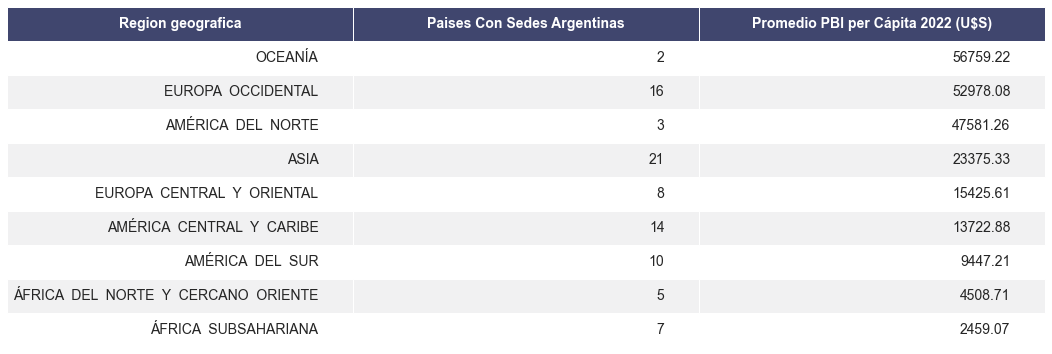
\includegraphics[width=1.0\textwidth]{TABLARegion.png}
  \caption{ Cantidad de sedes argentinas y promedio PBI para  cada region}
  \label{fig:Tabla 1}
\end{figure}

\vspace{12pt}

En tercera instancia, nos planteamos la siguiente pregunta con respecto a las redes sociales: ¿Cuán variado es, en cada país, el tipo de redes sociales que utilizan las sedes?. Para abordar esta interrogante de manera precisa, se construyó una tabla, se puede consultar en el anexo como 'redes\_por\_pais.csv', que muestra los nombres de los países y la cantidad de redes sociales utilizadas por sus sedes. Al analizar esta tabla, se observó que algunos países como Bélgica y Estados Unidos tienen la máxima cantidad de redes sociales, alcanzando un total de 6. Por otro lado, se identificó que países como Argentina y Haití no tienen presencia en redes sociales en sus sedes.

\vspace{0.1cm}

Por ultimo, tenemos una tabla, 'pais\_sede\_red.csv' en el anexo, donde se han registrado las redes sociales de cada país junto con sus respectivas URL. Se observa que la mayoría de los países cuentan con presencia en Facebook, seguido por Twitter y YouTube, mientras que LinkedIn y Flickr tienen una menor presencia en comparación


\subsection{Gráficos} \vspace{0.3cm}

Existen otras formas de visualizar datos las cuales mejoran la comprensión de la información. En este trabajo, se realizaron 3 tipos de gráfico, adecuados a los datos, histograma, boxplot, y scatter plot con el fin de entender más aquello que las tablas dicen.
A continuación, en el gráfico de cantidad de sedes por región se puede observar que América del sur es la región con mayor cantidad de sedes, mientras que Oceanía es la que menos posee.

\vspace{12pt}

\begin{figure}[h]
  \centering
  \includegraphics[width=1\textwidth]{bar_region.png}
  \caption{ Cantidad de sedes por region}
  \label{fig:Tabla 2}
\end{figure}

\vspace{12pt}

En el gráfico, se puede ver que Oceanía tiene la mediana más alta en relación con el PBI, mientras que África subsahariana tiene la mediana más baja. Por otro lado, se observa que Europa occidental tiene la sede con el PBI más grande, se puede ver claramente por el outlier que posee, el cual se encuentra más a la derecha en el grafico que los demás. También, podemos destacar que la mediana de Oceania, Ámerica del Norte y Europa Occidental es bastante similar, sin embargo, podemos ver que estos ulitmos dos presentan un "rango" de Pbi mucho más amplio. \par
Consideramos que el boxplot con todas las regiones juntas no aportaba toda la claridad necesaria, en particular, mirando aquellas dos regiones con el menor pbi. Por esto, se realizó otro grafico enfocado en África del norte y cercano oriente y  África subsahariana. A continuación, se pueden ver ambos.

\newpage

\begin{figure}[!]
  \centering
  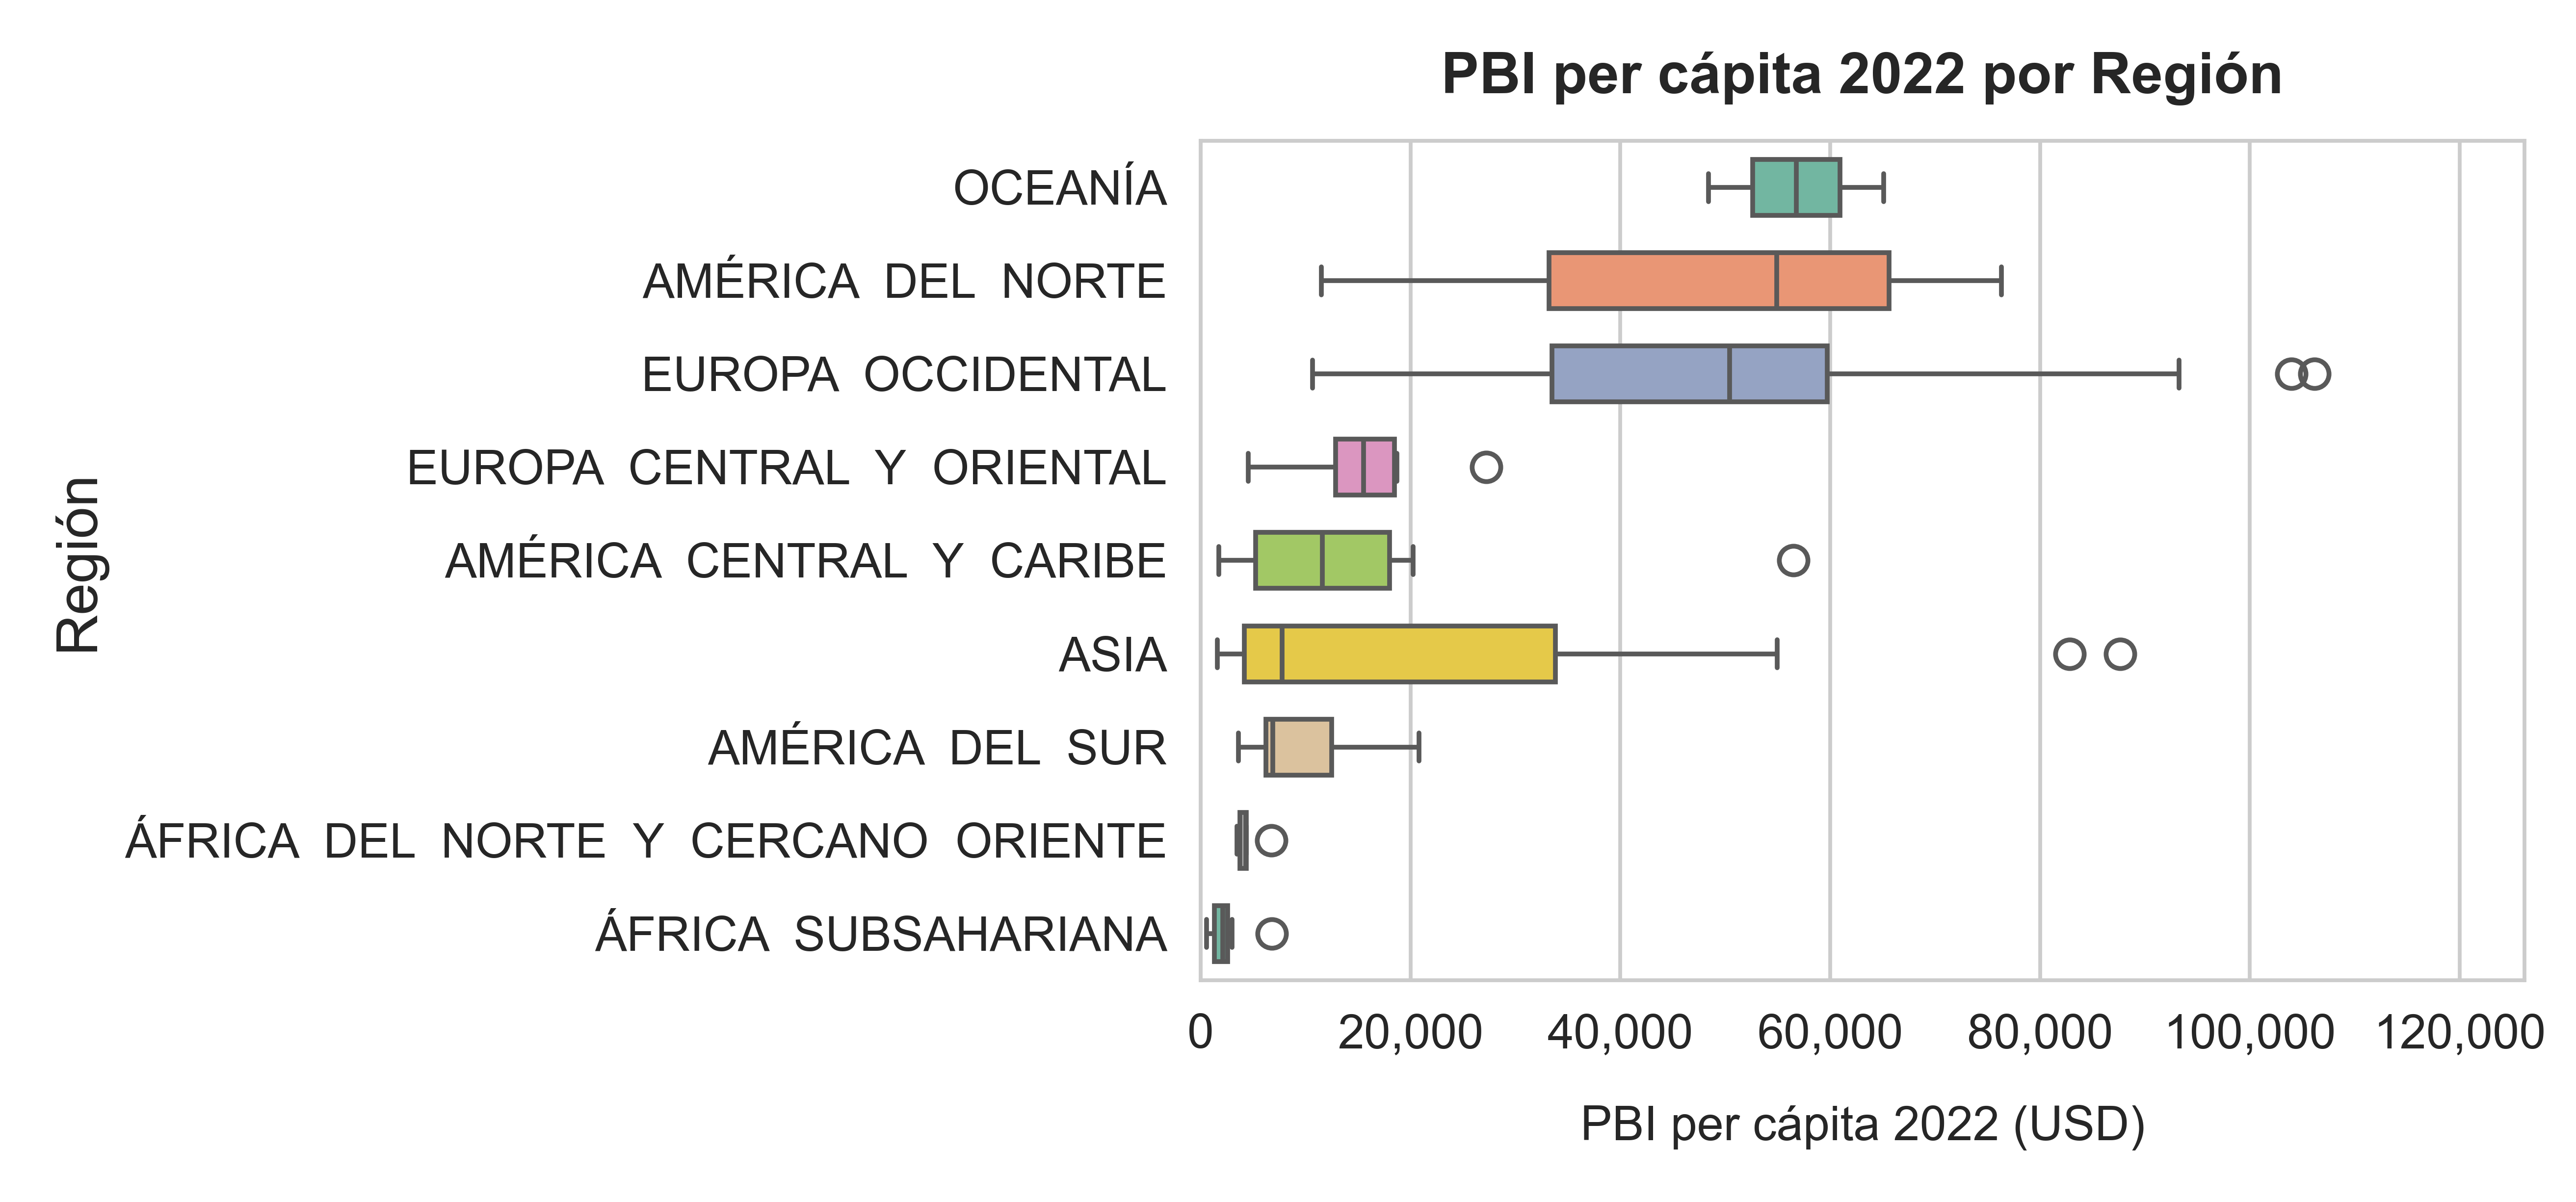
\includegraphics[width=1\textwidth]{boxplot_regiones.png}
  \caption{Pbi por región donde Argentina tiene una sede}
  \label{fig:Tabla 2}
\end{figure}

\begin{figure}[!] %% El !, obliga a la imagen a quedarse donde quieras
  \centering
  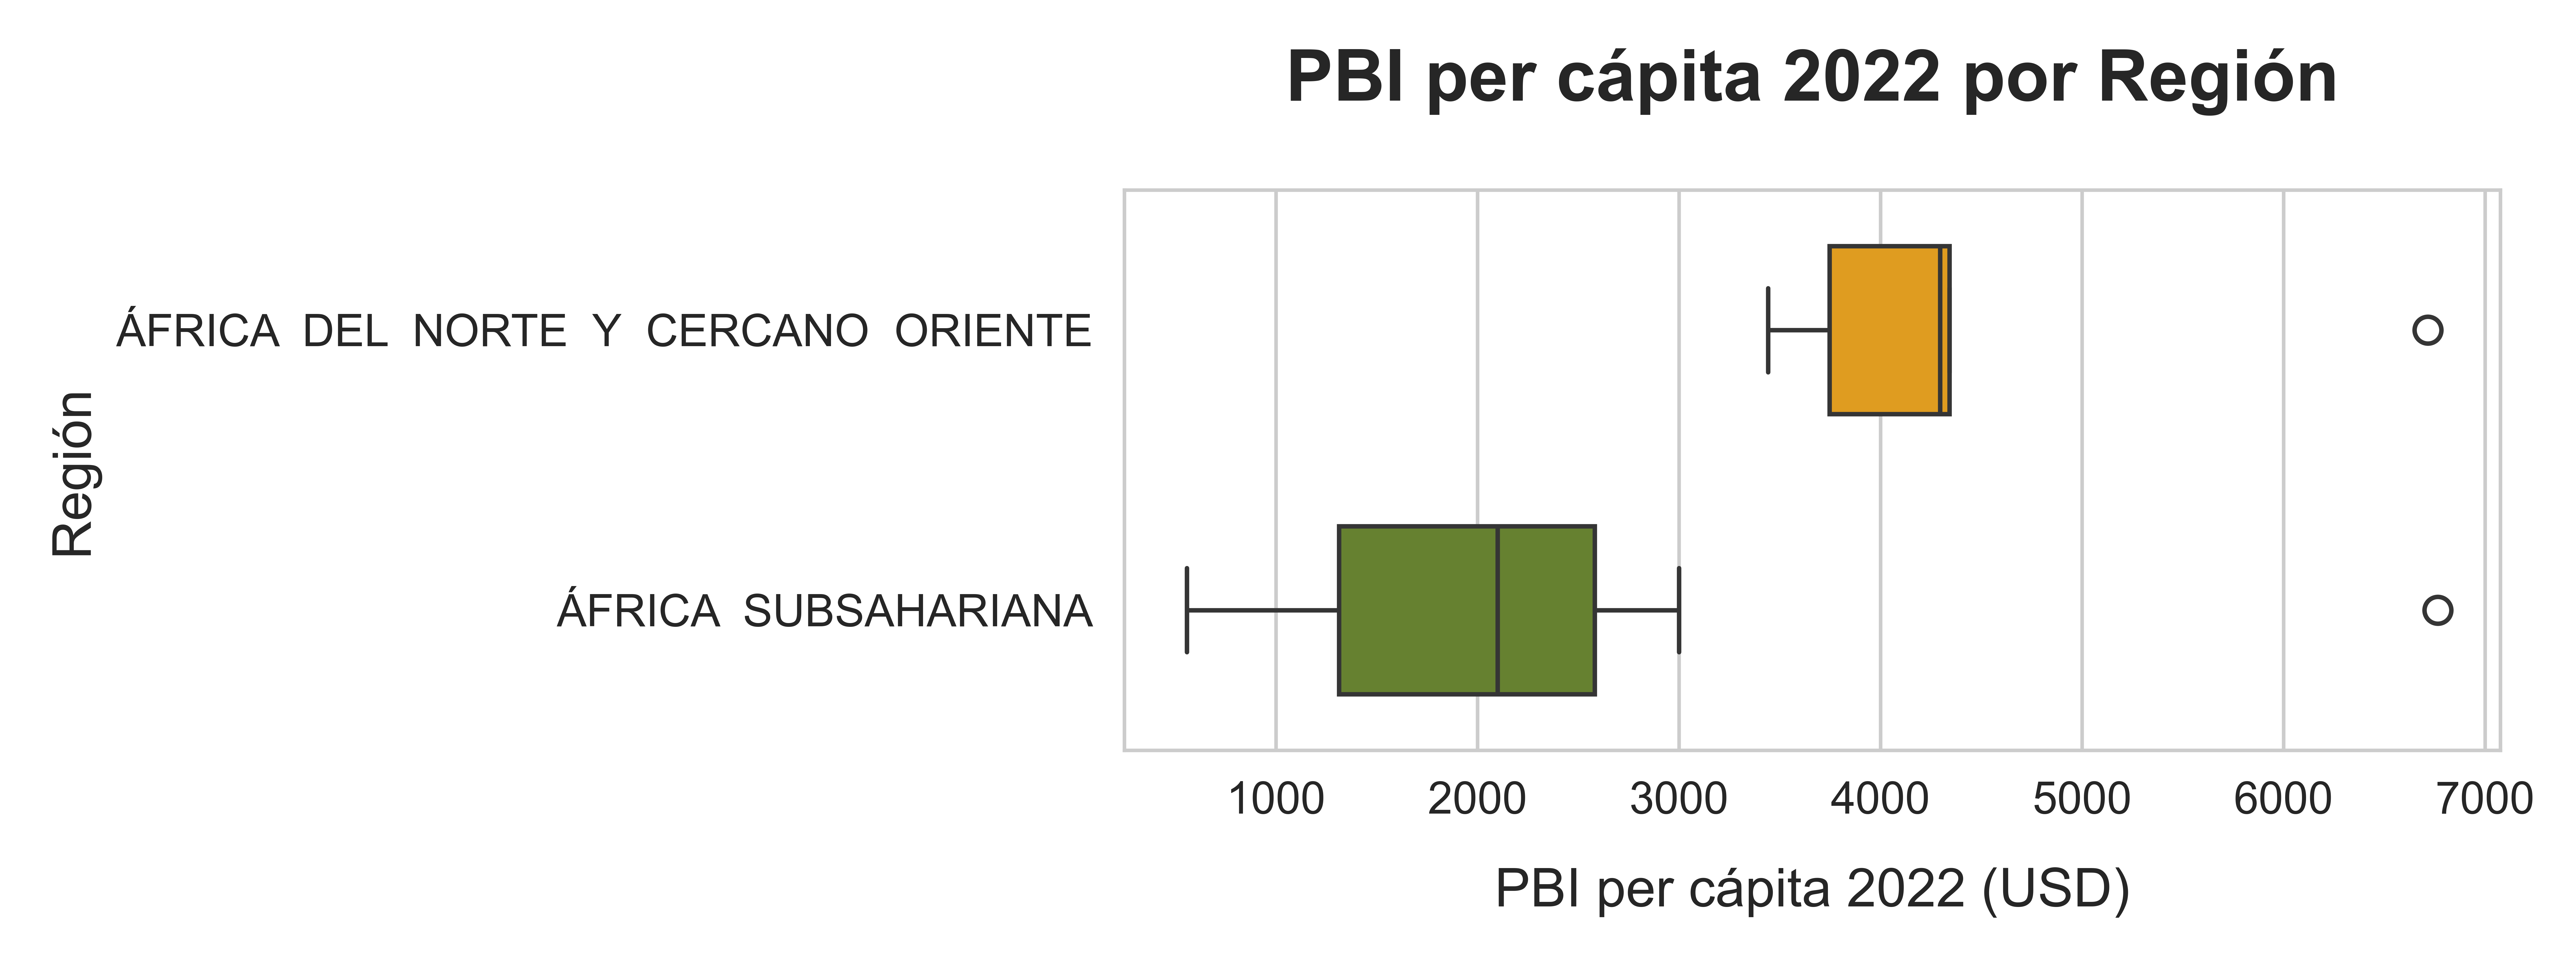
\includegraphics[width=1\textwidth]{boxplot_ultimas.png}
  \caption{ Pbi por region donde Argentina tiene una sede, en este grafico solo se muestra dos las regiones con menor PBI }
  \label{fig:Tabla 2}
\end{figure} \vspace{0.1cm}

Siguiendo con el último gráfico, se puede observar que los países que no tienen sedes  poseen  diversos  niveles de PBI. Por un lado, hay países con valores altos de PBI, mientras que también se encuentran países con PBI bajos. Esto nos lleva a pensar que la cantidad de sedes no es un factor que influya en el PBI, consideremos mejor, comparar el promedio entre aquellos paises que tienen presencia Argentina contra aquellos que no. 

\newpage

\begin{figure}[!] %% El !, obliga a la imagen a quedarse donde quieras
  \centering
  \includegraphics[width=1\textwidth]{plot_pbi.png}
  \caption{ Pbi por region donde Argentina tiene una sede, en este grafico solo se muestra dos las regiones con menor PBI }
  \label{fig:Tabla 2}
\end{figure} \vspace{0.1cm}


\subsection{Influencia de la Presencia Argentina} \vspace{0.3cm}

Como vimos antes, no pudimos terminar de determinar si la cantidad de sedes total tenia una influencia directa sobre el Pbi per Capita de un pais. Entonces, reformulemos nuestra pregunta un poco y veamos también si la muestra de paises por ejemplo con 11 sedes, por ejemplo, es significativa.

\newpage

\begin{figure}[h!]
  \centering
  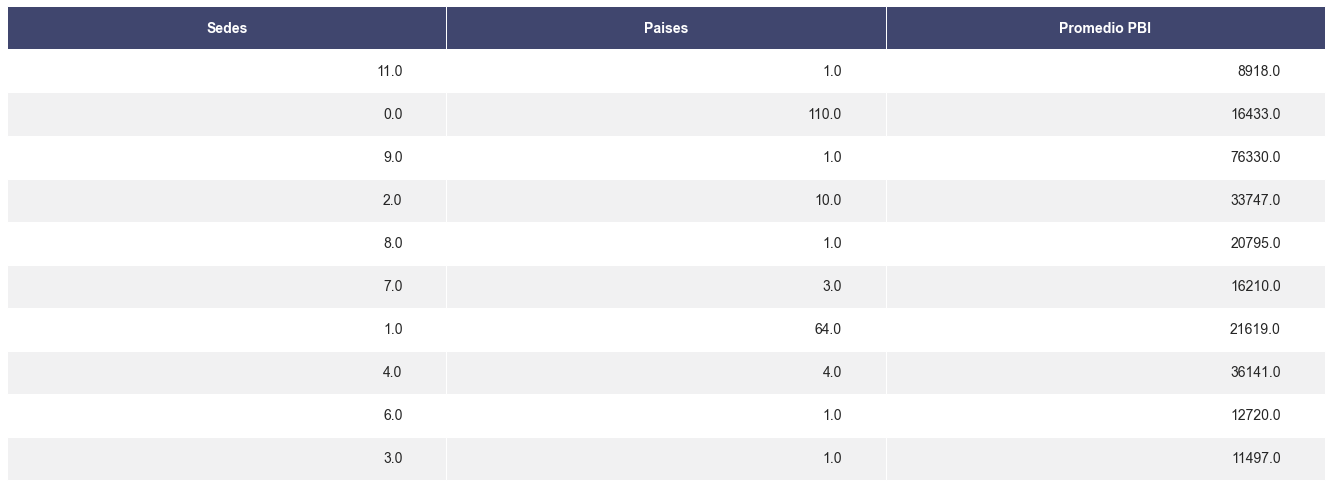
\includegraphics[width=1\textwidth]{TABLAConclusion1.png}
  \caption{La tabla muestra la cantidad de paises con determinada cantidad de sedes y el pbi promedio de estos }
  \label{fig:Tabla Conclusion}
\end{figure} \vspace{0.1cm}

Se puede empezar a vislumbrar que en las filas con una muestra signficativa de paises hay un patrón... 

\begin{figure}[h!]
  \centering
  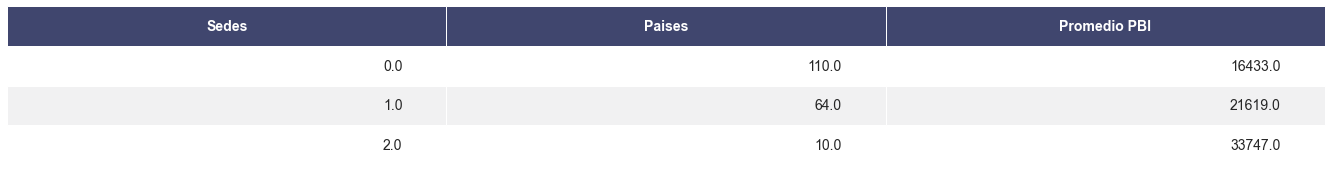
\includegraphics[width=1\textwidth]{TABLAConclusion.png}
  \caption{Muestra del pbi promedio por cantidad de sedes donde hay más de 10 paises }
  \label{fig:Tabla Conclusion}
\end{figure} \vspace{0.1cm}

Ahora si, todo parece indicar que la presencia de sedes argentinas influye de manera positiva en el pbi. Veamos también, solamente para dejar en claro esto la comparación entre el Pbi promedio de aquellos paises sin presencia Argentina contra aquellos con. En este, se verá claramente una tendencia que nos permitirá arribar a nuestro objetivo, encontrar una relación ente la cantidad de sedes argentinas y el Pbi.

\begin{figure}[h!]
  \centering
  \includegraphics[width=1\textwidth]{plot_conclusion.png}
  \caption{0 y 1 indican la presencia de sede}
  \label{fig: 0 y 1 indican la presencia de sedes}
\end{figure} \vspace{0.1cm}

\newpage

\section{Conclusiones} \vspace{0.3cm}

A raiz de lo visto en la sección anterior, 'Analisis de Datos', consideramos que la respuesta a nuestro problema es clara. Aquellos paises que poseen alguna sede Argentina, en promedio, tienen un Pbi mayor que aquellos que no. Más aún, vimos que cuando dividimos a los paises en cantidad de sedes por paises y tomamos aquellos grupos con muestras de paises significativas, el Pbi tendia también a ser mayor. Como todo, hay paises que se escapan de estas métricas, como por ejemplo, Monaco quien no posee sedes y aún asi es el país con mayo Pbi per cápita del mundo. También, creemos que esta tendencia se debe a que argentina tiene una cantidad baja, por no decir nula, de sedes en áfrica, mientras que en regiones historicamente mas ricas como europa occiddental o norteamerica tiene una fuerte presencia.


\end{document}